\section{Enabling COMPSs Monitor}
\label{sec:Monitor}

\subsection{Configuration}

As supercomputer nodes are connection restricted, the better way to enable the \textit{COMPSs Monitor} is from the users local machine. 
To do so please install the following packages:
\begin{itemize}
 \item COMPSs Runtime
 \item COMPSs Monitor
 \item sshfs
\end{itemize}

For further details about the COMPSs packages installation and configuration please refer to the \textit{COMPSs Installation Manual} 
available at our webpage \url{http://compss.bsc.es} . If you are not willing to install COMPSs in your local machine please consider
to download our Virtual Machine available at our webpage. 
\newline

Once the packages have been installed and configured, users need to mount the sshfs directory as follows. The \verb|SC_USER| stands for 
your supercomputer's user, the \verb|SC_ENDPOINT| to the supercomputer's public endpoint and the \verb|TARGET_LOCAL_FOLDER| to 
the local folder where you wish to deploy the supercomputer files):

\begin{lstlisting}[language=bash]
compss@bsc:~$ scp $HOME/.ssh/id_dsa.pub ${SC_USER}@mn1.bsc.es:~/id_dsa_local.pub
compss@bsc:~$ ssh SC_USER@SC_ENDPOINT 
                  "cat ~/id_dsa_local.pub >> ~/.ssh/authorized_keys; 
                  rm ~/id_dsa_local.pub"
compss@bsc:~$ mkdir -p TARGET_LOCAL_FOLDER/.COMPSs
compss@bsc:~$ sshfs -o IdentityFile=$HOME/.ssh/id_dsa -o allow_other 
                   SC_USER@SC_ENDPOINT:~/.COMPSs 
                   TARGET_LOCAL_FOLDER/.COMPSs
\end{lstlisting}

Whenever you wish to unmount the sshfs directory please run:

\begin{lstlisting}[language=bash]
compss@bsc:~$ sudo umount TARGET_LOCAL_FOLDER/.COMPSs
\end{lstlisting}


\subsection{Execution}
Access the COMPSs Monitor through its webpage (\url{http://localhost:8080/compss-monitor} by default) and log in with the 
\verb|TARGET_LOCAL_FOLDER| to enable the COMPSs Monitor for MareNostrum. 

\colorComment{Please remember that to enable \textbf{all} the COMPSs Monitor features applications must be ran with the \textit{-m}
flag. For further information please check the \textit{COMPSs User Manual: Application Execution} available at our webpage
\url{http://compss.bsc.es} .}

\newpage

~ \newline

Figure \ref{fig:mn_monitor1} illustrates how to login and Figure \ref{fig:mn_monitor2} shows the COMPSs Monitor
main page for an application run inside a Supercomputer. 

~ \newline

\begin{figure}[!htb]
  \centering
    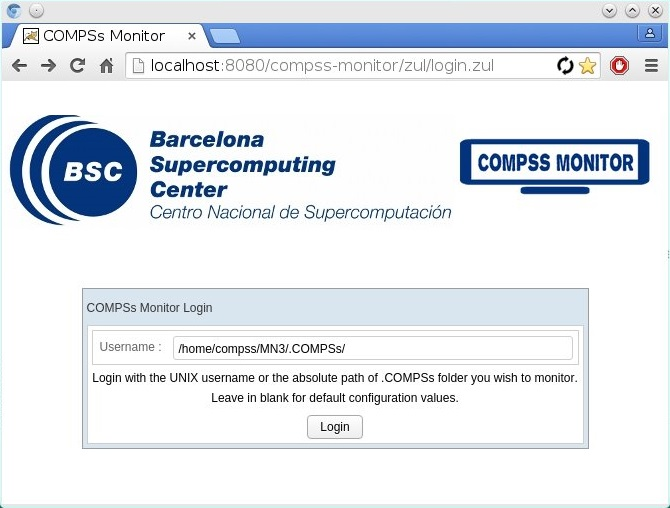
\includegraphics[width=0.75\textwidth]{./Sections/6_Monitor/Figures/mn_monitor1.jpeg}
    \caption{COMPSs Monitor login for Supercomputers}
    \label{fig:mn_monitor1}
\end{figure}

\newpage

\begin{figure}[!htb]
  \centering
    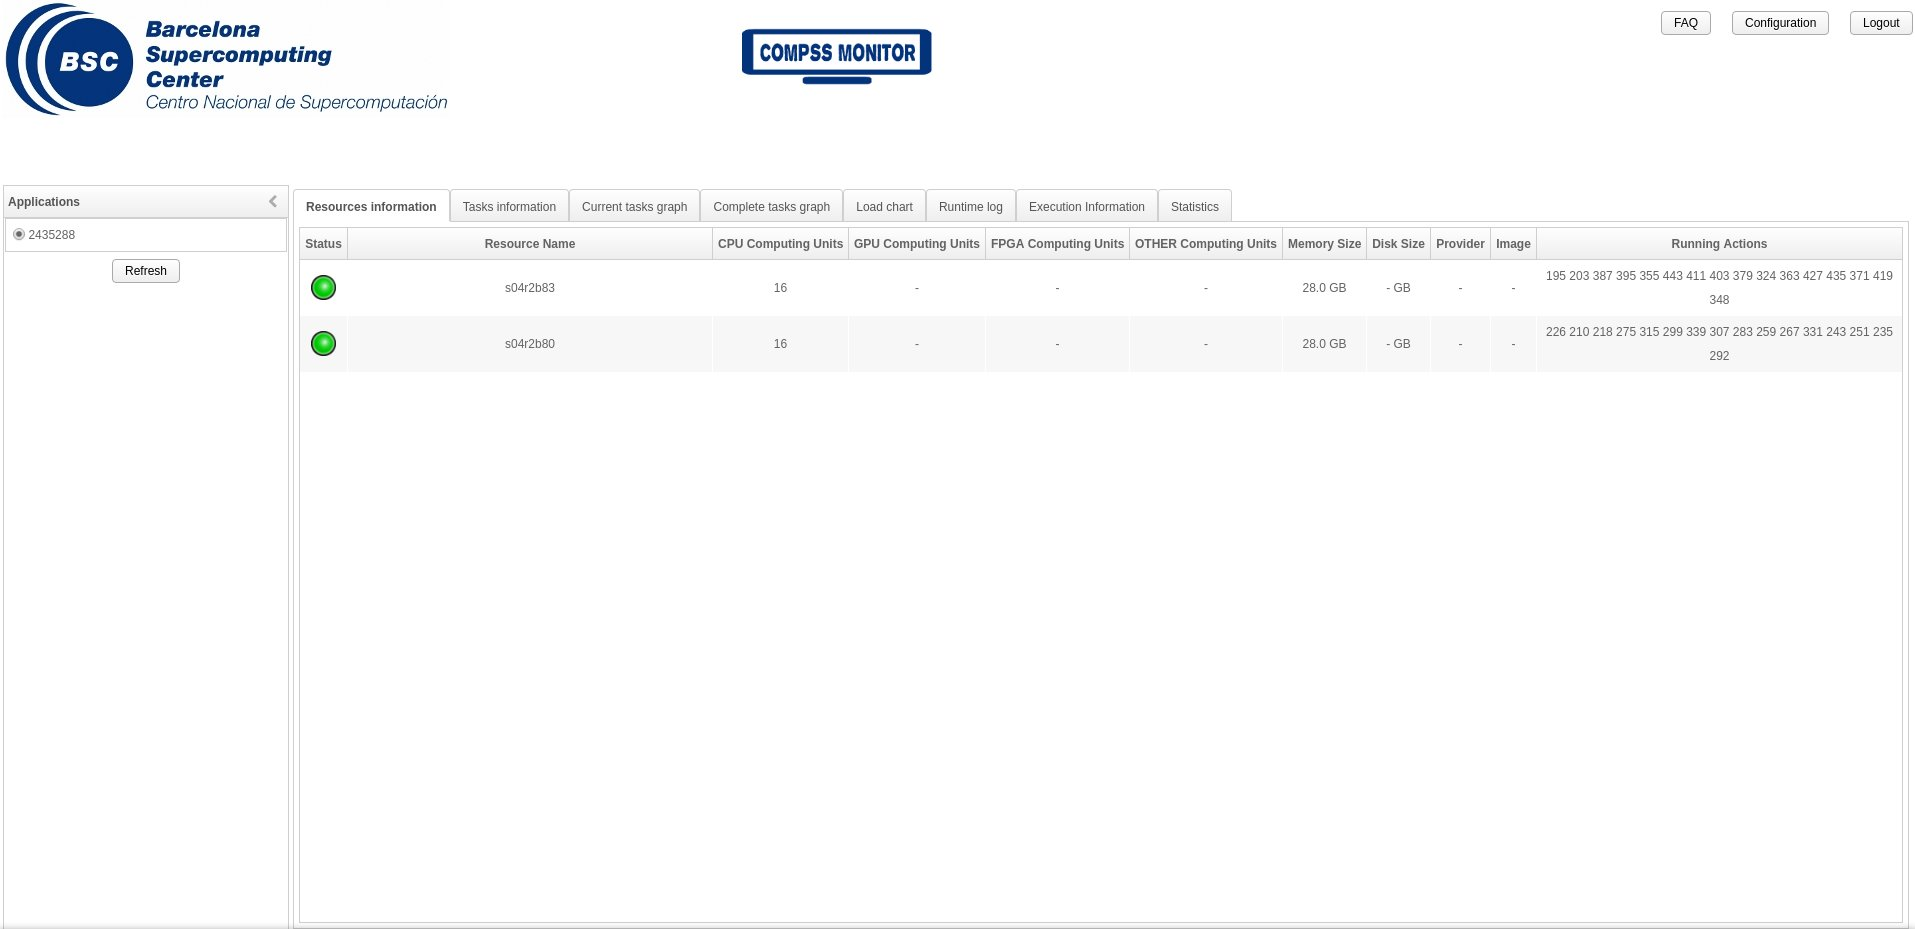
\includegraphics[width=\textwidth]{./Sections/6_Monitor/Figures/mn_monitor2.jpeg}
    \caption{COMPSs Monitor main page for a test application at Supercomputers}
    \label{fig:mn_monitor2}
\end{figure}
